\documentclass[notheorems,mathserif,table,Singapore]{beamer}

\useoutertheme[height=0.1\textwidth,width=0.15\textwidth,hideothersubsections]{sidebar}
\usecolortheme{seahorse}                       % Outer color themes, 其他选择: whale, seahorse, dolphin . 换一个编译看看有什么不同.
\usecolortheme{lily}                           % Inner color themes, 其他选择: lily, orchid
\useinnertheme[shadow]{rounded}                % 对 box 的设置: 圆角、有阴影.
\setbeamercolor{sidebar}{bg=blue!60}           % sidebar的颜色, 50%的蓝色.
%\setbeamercolor{background canvas}{bg=blue!9} % 背景色, 9%的蓝色. 去掉下一行, 试一试这个.
\setbeamertemplate{background canvas}[vertical shading][bottom=white,top=structure.fg!20] %%背景色, 上25%的蓝, 过渡到下白.
\usefonttheme{serif}                          % 字体. 个人偏好有轮廓的字体. 去掉这个设置编译, 就看到不同了.
%\setbeamertemplate{navigation symbols}{}      %% 去掉页面下方默认的导航条.
%%------------------------常用宏包---------------------------------------------------------------------
%%注意, beamer 会默认使用下列宏包: amsthm, graphicx, hyperref, color, xcolor, 等等
\usepackage[slantfont,boldfont]{xeCJK}        %使用xeCJK宏包
\usepackage{hyperref}
\setCJKmainfont{WenQuanYi Zen Hei Mono}
\setCJKmainfont[BoldFont=Adobe Heiti Std,ItalicFont=Adobe Kaiti Std]{Adobe Song Std} %设置正文为宋体,粗体使用黑体,斜体使用楷体
\setCJKmonofont{Adobe Song Std}                                                      %设置等距字体
\setCJKsansfont[BoldFont=Adobe Heiti Std]{Adobe Kaiti Std}                           %设置无衬线字体
%%-----------------------设置英文字体-----------------------------------------------------------------------------------------
\setmainfont[Mapping=tex-text]{WenQuanYi Zen Hei}      %英文衬线字体
\setsansfont[Mapping=tex-text]{WenQuanYi Zen Hei}      %英文无衬线字体
\setmonofont[Mapping=tex-text]{WenQuanYi Zen Hei}      %英文等宽字体
%%%%----------重定义中文字体%%%%---------------
\setCJKfamilyfont{song}{Adobe Song Std}
\setCJKfamilyfont{hei}{Adobe Heiti Std}
\setCJKfamilyfont{kai}{Adobe Kaiti Std}
\setCJKfamilyfont{fs}{Adobe Fangsong Std}
%%-------------------------------------
\newcommand{\song}{\CJKfamily{song}}
\newcommand{\hei}{\CJKfamily{hei}}
\newcommand{\kai}{\CJKfamily{kai}}
\newcommand{\fs}{\CJKfamily{fs}}
\punctstyle{kaiming} %开明式标点格式
\linespread{1.5}   % 1.5倍行距
%%%%%%%%%%%%%%%%%%%%%%%%%%%%%%%%%%%%%%%%%%%%%%%%%%%%%%%%%%%%%%%%%%%%%%%%%%%%%%%%%%%%%%%%%%%%%%%%%%%%%%%%
\begin{document}
%%----------------------- Theorems ---------------------------------------------------------------------
\newtheorem{theorem}{定理}
\newtheorem{definition}{定义}
\newtheorem{lemma}{引理}
%%----------------------------------------------------------------------------------------------------
\title{\hei 测试代码}
\subtitle{\hei test 与 helloworld}
\author[\textcolor{white}{\song 冯海雄}]{{\song 作者~~\textcolor{olive}{冯海雄}}}
\institute{\textcolor{violet}{程序中心研发部大数据解决方案组}}
\date{2014年10月10日}
\frame{ \titlepage }
%%---------------------------------------------------------------------------------------------------
%\section*{目录}
%\frame{\frametitle{目录}\tableofcontents}
%%===================================================================================================
\section{第一部分}
%任意两行单列线表示一张ppt
%%---------------------------------------------------------------------------------------------------
\begin{frame}
\frametitle{第一页}
\begin{itemize}
 \item 第一条
 \item 第二条
 \item 第三条
\end{itemize}
\end{frame}
%%---------------------------------------------------------------------------------------------------
\section{第二部分}
\begin{frame}
\frametitle{第二页}

\begin{itemize}
\item 1天标准
\item 7天标准
\item 14天标准
\item 30天标准
\end{itemize}
\end{frame}
\begin{frame}
\frametitle{第三页}
有三个统计周期分别是:
\begin{itemize}
\item 一个自然日
\item 一个自然周
\item 一个自然月
\end{itemize}
\end{frame}
%%---------------------------------------------------------------------------------------------------
\section{第三部分}
\begin{frame}
\frametitle{第四页}

\begin{itemize}
\item \small 数据
\end{itemize}
\begin{table}[h]\tiny
\begin{tabular}{l c c c c c c r}
\hline
date &\ & product & \ & key &\ & platForm & interval\\
\hline
1		 &\  & 104513 &\ 	& 503927 &\ 	&  iphone &0\\
2           &\  & 104513 &\    & 503927 &\ 	&  iphone &1\\
3 	         &\  & 104513 &\    & 503927 &\ 	&  iphone & 1\\
4           &\  & 104513 &\    & 503927 &\ 	&  iphone &3\\
5         &\  & 104513 &\    & 503927 &\ 	&  iphone &7\\
6         &\  & 104513 &\    & 503927 &\ 	&  iphone &37\\
\hline
\end{tabular}
\end{table}
\end{frame}

\begin{frame}[shrink=10]
\frametitle{第五页}
\begin{itemize}
\item \small 数据
\end{itemize}
\begin{table}[h]\tiny
\begin{tabular}{l c c c c c c r}
\hline
date &\ & product & \ & key &\ & platForm & interval\\
\hline
1		 &\  & 104513 &\ 	& 503927 &\ 	&  iphone &0\\
2   &\  & 104513 &\    & 503927 &\ 	&  iphone &1\\
3 	 &\  & 104513 &\    & 503927 &\ 	&  iphone & 1\\
6   &\  & 104513 &\    & 503927 &\ 	&  iphone &3\\
30   &\  & 104513 &\    & 503927 &\ 	&  iphone &7\\
15 &\  & 104513 &\    & 503927 &\ 	&  iphone &37\\
\hline
\end{tabular}

\end{table}
\begin{itemize}
\item \small 根据间隔天数分类
\end{itemize}
\begin{table}\tiny
\begin{tabular}{c  c c c c c c }
\hline
product & key & channelId &  loginState01 & loginState07 & loginState14 & loginState30 \\
\hline
104513 & 503927 & 1   &       1      &     1        &    1  &    1\\ 
104513 & 503927 & 1   &       2      &     2        &    2  &    2\\  
104513 & 503927 & 1   &       2      &     2        &    2  &    2\\   
104513 & 503927 & 1   &       3      &     2        &    2  &    2\\ 
104513 & 503927 & 1   &       3      &     2        &    2  &    2\\ 
104513 & 503927 & 1   &       3      &     3        &    3  &    3\\ 
\hline
\end{tabular}
\end{table}
\end{frame}
\begin{frame}
\frametitle{第六页}
\begin{itemize}
\item \small 分类
\end{itemize}
\begin{table}\tiny
\begin{tabular}{c  c c c c c c }
\hline
product & key & channelId &  loginState01 & loginState07 & loginState14 & loginState30 \\
\hline
104513 & 503927 & 1   &       1      &     1        &    1  &    1\\ 
104513 & 503927 & 1   &       2      &     2        &    2  &    2\\  
104513 & 503927 & 1   &       2      &     2        &    2  &    2\\   
104513 & 503927 & 1   &       3      &     2        &    2  &    2\\ 
104513 & 503927 & 1   &       3      &     2        &    2  &    2\\ 
104513 & 503927 & 1   &       3      &     3        &    3  &    3\\ 
\hline
\end{tabular}
\end{table}
\begin{itemize}
\item 结果
\end{itemize}
\begin{table}\tiny
\begin{tabular}{c c c c c c c c c}
\hline
product & key & channelId &  loginState01 & loginState07 & loginState14 & loginState30\\
\hline
104513 & 503927 & 1   &       1      &     1        &    1  &    1 \\ 
\hline
\end{tabular}
\end{table}
\end{frame}
\begin{frame}
\frametitle{第7页}

\begin{itemize}
\item 结果
\end{itemize}
\begin{table}\tiny
\begin{tabular}{c c c c c c c c c}
\hline
product & key & channelId &  loginState01 & loginState07 & loginState14 & loginState30\\
\hline
104513 & 503927 & 1   &       1      &     1        &    1  &    1 \\ 
\hline
\end{tabular}
\end{table}
\begin{itemize}
\item 周期
\end{itemize}
\begin{table}\tiny
\begin{tabular}{c c c c c c c c c}
\hline
product  & loginCnt &  loginNew & loginLive01 & loginLive07 & loginLive14 &LoginLive30\\
\hline
104513   & 1         &        1  &     0       &    0        &    0        & 0    \\ 
\hline
\end{tabular}
\end{table}
\end{frame}

%%---------------------------------------------------------------------------------------------------
\begin{frame}\frametitle{定理}
\begin{lemma}[1]
这是一个定理,引理类似。
\end{lemma}
\pause                       % 这里会暂停一下,pagedown会接着出现下面的式子
\begin{displaymath}             %这个不用解释了吧
1+1=2
\end{displaymath}
\begin{equation}
1+1=2
\end{equation}
\end{frame}
%%================================================================================新目录
\section*{未尽的思考}
%---------------------------------------------------------------------------------------------------
\begin{frame}\frametitle{插个图}
\begin{figure}[!htbp]
\centering
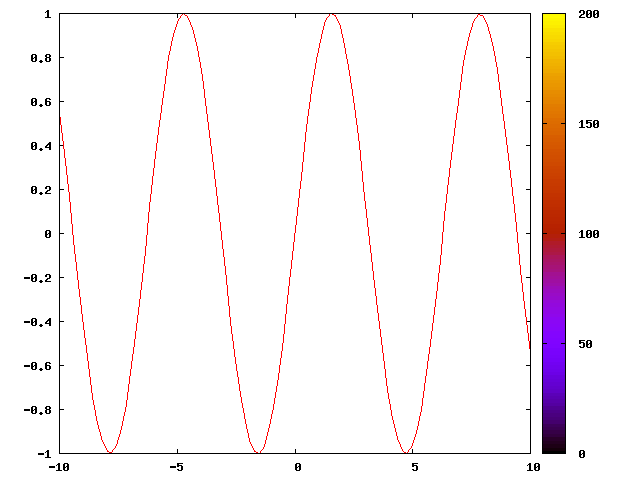
\includegraphics[width=4.00cm,height=2.10cm]{test}
\caption{一个图}
\end{figure}
\end{frame}
%%---------------------------------------------------------------------------------------------------

%%---------------------------------------------------------------------------------------------------
\begin{frame}\frametitle{插个表}
一个表.
 \begin{table}
  \centering \addtolength{\tabcolsep}{1mm}
 \begin{tabular}{ccccccccc}
   \hline
        & 1 & 2 & 3 & 4 & 5 & 6 & 7 & 8 \\
   \hline
   1 &         &       &          &       &       &       &       &  \\
   2 & $c$     &       &          &       &       &       &       &  \\
   3 & $c$     & $c $  &          &       &       &       &       &  \\
   4 & $a$     & $a,c$ & $a $     &       &       &       &       &  \\
   5 & $a,b,c$ & $a,b$ & $a,b,c$  & $b,c$ &       &       &       &  \\
   6 & $a,c$   & $a,c$ & $a,c$    & $c $  & $b,c$ &       &       &  \\
   7 & $a,b,c$ & $a,b$ & $a,b,c$  & $b,c$ &       & $b,c$ &       &  \\
   8 & $a,c$   & $a,c$ & $a,c$    & $c$   & $b,c$ &       & $b,c$ &  \\
   \hline
 \end{tabular}\label{dismatrix}
 \end{table}
\end{frame}
%%---------------------------------------------------------------------------------------------------
\begin{frame}\frametitle{就这样吧}
就这样吧,遗计。
\end{frame}
%================================================================================新目录
\section{参考文献}
%---------------------------------------------------------------------------------------------------
\begin{frame}\frametitle{参考文献}
[1] A\newline
[2] B
\end{frame}
%%%%%%%%%%%%%%%%%%%%%%%%%%%%%%%%%%%%%%%%%%%%%%%%%%%%%%%%%%%%%%%%%%%%%%%%%%%%%%%%%%%%%%%%%%%%%
\section{致谢}
%---------------------------------------------------------------------------------------------------

\begin{frame}\frametitle{致谢}
\centering{谢谢欣赏}
\end{frame}
%%%%%%%%%%%%%%%%%%%%%%%%%%%%%%%%%%%%%%%%%%%%%%%%%%%%%%%%%%%%%%%%%%%%%%%%%%%%%%%%%%%%%%%%%%%%%%
\end{document}
